%\section{Electroweak $\text{ZZ}jj$ Production and Search for aQGCs}
%\label{sec:llvvjj}

\subsection{Constraints on Anomalous Quartic Gauge Couplings}
\label{subsec:aqgc_limits}

The measurement of $\text{ZZ}jj$ production is sensitive to the VBS processes, which offer a unique probe of quartic electroweak gauge boson interactions. In the context of the SMEFT framework, such effects are parameterised by extending the SM Lagrangian with higher-dimensional operators as follows: 
\begin{equation}
\mathcal{L}_\text{SMEFT} = \mathcal{L}_\text{SM} + \sum_i \frac{f_{\text{T}i}}{\Lambda^4} \mathcal{O}_{\text{T}i}^{(8)}.
\label{eqn:eft}
\end{equation}
Dimension-8 operators are considered here, as they directly contribute to quartic gauge couplings, which do not arise at lower dimensions~\cite{Eboli2016}.

As in Equation~\eqref{eqn:eft}, the SMEFT Lagrangian includes dimension-eight operators $\mathcal{O}_{\text{T}i}$, each associated with a Wilson coefficient $f_{\text{T}i}/ \Lambda^4$, where $i = 0, 1, \ldots, 9$, to distinguish them from the $C_i$ coefficients used for aTGCs in Section~\ref{sec:aTGC}.

%%%%%%%%%%%%%
$\text{ZZ}jj$ production provides direct sensitivity to the $\text{ZZWW}$ and $\text{ZZZZ}$ quartic vertices. In the SM, the cross-section contribution from these vertices is small. However, physics beyond the SM (BSM) could manifest as Anomalous Quartic Gauge Couplings (aQGCs), leading to a significant enhancement of the cross-section at high energy scales.

The aQGCs are parameterised using the Standard Model Effective Field Theory (SMEFT) framework. This analysis considers dimension-8 operators, specifically the transversal operators $\text{T}0$ through $\text{T}9$, which induce quartic couplings without modifying triple gauge couplings.

The most sensitive observable for detecting aQGCs is the transverse mass of the $\text{ZZ}$ system (see the distribution in Figure~\ref{fig:mTZZ-aQGC}), defined as:
\begin{equation}
    m_{\text{T}}^{\text{ZZ}} = \sqrt{ \left( \sqrt{m_{\text{Z}}^2 + (p_{\text{T}}^{\ell\ell})^2} + \sqrt{m_{\text{Z}}^2 + (E_{\text{T}}^{\text{miss}})^2} \right)^2 - \left| \vec{p}_{\text{T}}^{\ell\ell} + \vec{E}_{\text{T}}^{\text{miss}} \right|^2 }.
\end{equation}
The presence of aQGCs would appear as an excess of events in the high-$m_{\text{T}}^{\text{ZZ}}$ tail.

\begin{figure}
    \centering
    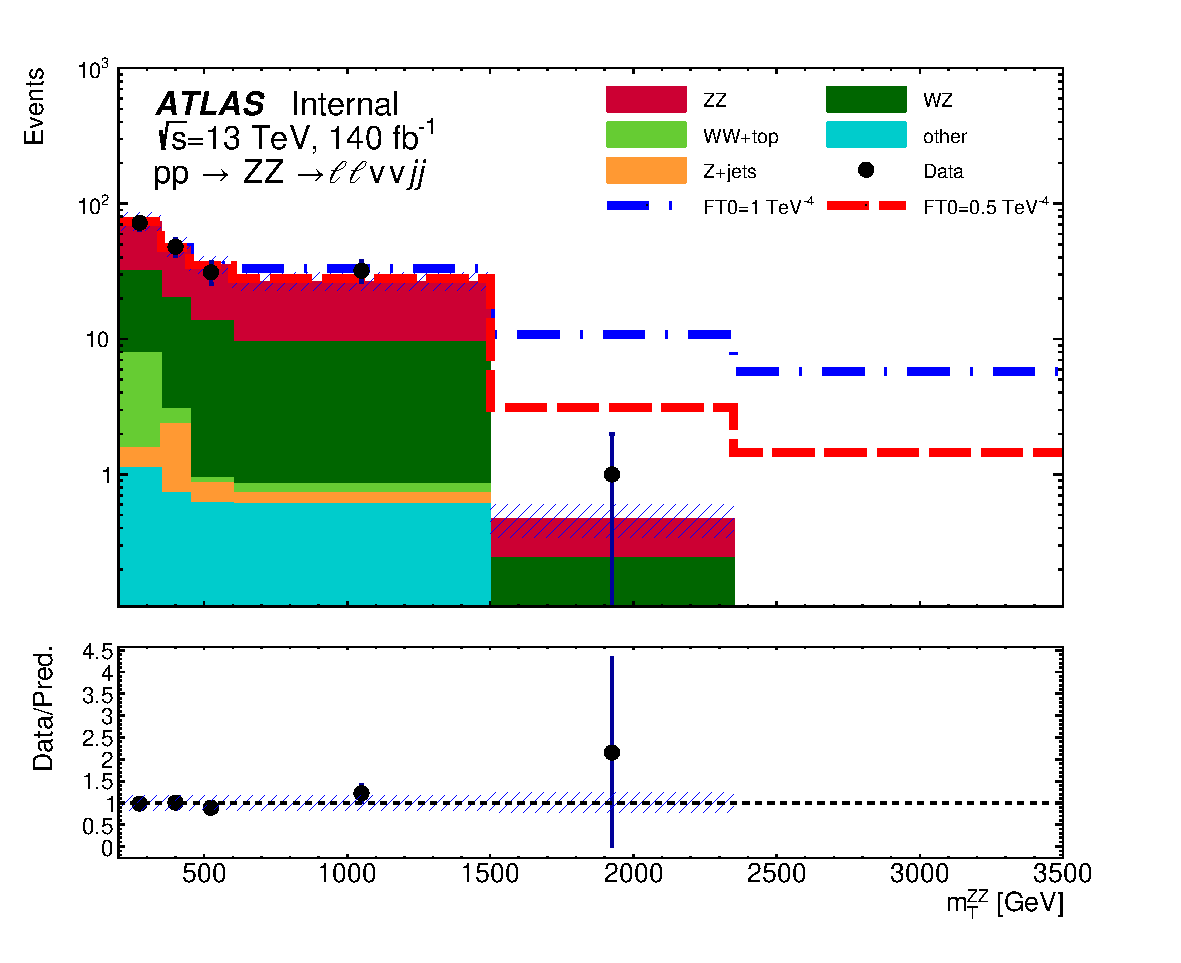
\includegraphics[width=0.6\linewidth]{figures/ch5-llvv/aTGC-aQGC/FT0_mTZZ_events.pdf}
    \caption{Comparison between data and MC predictions for the transverse mass of the $\text{ZZ}$ system, $m_{\text{T}}^{\text{ZZ}}$, at detector level. Predictions in the SMEFT framework for the $f_{\text{T}0}$ operator and two values of the Wilson coefficient are also shown.}
    \label{fig:mTZZ-aQGC}
\end{figure}

%\subsubsection{Limits on Wilson Coefficients}
The reconstructed transverse mass of the $\text{ZZ}$ system, $m_{\text{T}}^{\text{ZZ}}$, shown in Figure~\ref{fig:mTZZ-aQGC}, is used to extract limits on dimension-8 SMEFT operators. A binned likelihood fit to the $m_{\text{T}}^{\text{ZZ}}$ spectrum in the $\text{ZZ}jj$ signal region (SR) is performed to derive 95\% confidence level (CL) intervals for the Wilson coefficients $f_{\text{T}i}/\Lambda^4$ ($i = 0$--$9$). Systematic uncertainties are incorporated as nuisance parameters in the fit. The resulting limits are summarised in Table~\ref{tab:combined_run2_ZZjj_eft_intervals}, where each coefficient is varied individually while all others are set to zero.

To ensure the validity of the SMEFT expansion, unitarity-preserving cut-offs are applied to the BSM contributions by restricting $m_{\text{ZZ}} < E_{\text{c}}$, where $E_{\text{c}}$ denotes the energy cut-off scale.

\begin{table}[!htbp]
\centering
\scriptsize
\renewcommand{\arraystretch}{1.5}
\begin{tabular}{l c c c c c c}
\hline
\textbf{Wilson Coefficient} & 
\multicolumn{2}{c}{\textbf{No cut-off}} & 
\multicolumn{2}{c}{\textbf{$E_{\text{c}} = 1~\text{TeV}$}} & 
\multicolumn{2}{c}{\textbf{$E_{\text{c}} = 1.5~\text{TeV}$}} \\
\cline{2-7}
& \textbf{Expected} & \textbf{Observed} & 
  \textbf{Expected} & \textbf{Observed} & 
  \textbf{Expected} & \textbf{Observed} \\
\hline
$f_{\text{T}0}/\Lambda^4$ & $[-0.42,\ 0.40]$ & $[-0.50,\ 0.49]$ & $[-3.9,\ 3.8]$ & $[-4.9,\ 4.9]$ & $[-2.8,\ 2.6]$ & $[-4.0,\ 3.4]$ \\
$f_{\text{T}1}/\Lambda^4$ & $[-0.46,\ 0.46]$ & $[-0.56,\ 0.56]$ & $[-3.7,\ 3.6]$ & $[-4.6,\ 4.6]$ & $[-2.9,\ 2.8]$ & $[-3.8,\ 3.8]$ \\
$f_{\text{T}2}/\Lambda^4$ & $[-0.95,\ 0.93]$ & $[-1.1,\ 1.1]$ & $[-7.7,\ 7.6]$ & $[-9.8,\ 9.7]$ & $[-5.9,\ 5.6]$ & $[-7.7,\ 7.4]$ \\
$f_{\text{T}3}/\Lambda^4$ & $[-1.3,\ 1.3]$ & $[-1.6,\ 1.6]$ & $[-9.9,\ 9.9]$ & $[-13,\ 13]$ & $[-7.7,\ 7.4]$ & $[-10.0,\ 9.7]$ \\
$f_{\text{T}4}/\Lambda^4$ & $[-8.8,\ 8.5]$ & $[-11,\ 11]$ & $[-55,\ 54]$ & $[-69,\ 69]$ & $[-43,\ 41]$ & $[-56,\ 53]$ \\
$f_{\text{T}5}/\Lambda^4$ & $[-0.75,\ 0.71]$ & $[-0.89,\ 0.87]$ & $[-6.9,\ 6.7]$ & $[-8.7,\ 8.6]$ & $[-4.8,\ 4.4]$ & $[-6.2,\ 5.8]$ \\
$f_{\text{T}6}/\Lambda^4$ & $[-1.1,\ 1.1]$ & $[-1.4,\ 1.4]$ & $[-6.9,\ 6.9]$ & $[-8.9,\ 8.9]$ & $[-5.4,\ 5.3]$ & $[-7.1,\ 7.0]$ \\
$f_{\text{T}7}/\Lambda^4$ & $[-2.5,\ 2.4]$ & $[-3.0,\ 3.0]$ & $[-14,\ 14]$ & $[-18,\ 18]$ & $[-18,\ 18]$ & $[-22,\ 21]$ \\
$f_{\text{T}8}/\Lambda^4$ & $[-0.60,\ 0.60]$ & $[-0.74,\ 0.74]$ & $[-6.7,\ 6.7]$ & $[-8.7,\ 8.7]$ & $[-3.8,\ 3.8]$ & $[-4.9,\ 4.9]$ \\
$f_{\text{T}9}/\Lambda^4$ & $[-1.3,\ 1.3]$ & $[-1.6,\ 1.6]$ & $[-14,\ 14]$ & $[-18,\ 18]$ & $[-7.9,\ 7.9]$ & $[-10.0,\ 10.0]$ \\
\hline
\end{tabular}
\caption{\rm Expected and observed 95\% CL intervals for the dimension-8 Wilson coefficients in the 
$\text{ZZ}jj \to \ell\ell\nu\nu jj$ phase space, derived from a one-dimensional fit to the $m_{\text{T}}^{\text{ZZ}}$ spectrum. Results are shown for three EFT validity scenarios: without unitarisation, and with energy cut-offs at $1~\text{TeV}$ and $1.5~\text{TeV}$.}
\label{tab:combined_run2_ZZjj_eft_intervals}
\end{table}

The observed limits are consistent with zero for all operators. To further assess the validity of the EFT expansion, unitarity bounds are evaluated as a function of the energy cut-off scale $E_{\text{c}}$.

Figures~\ref{fig:fT0-fT1_zzjj_EFT} and~\ref{fig:fT2-fT9_zzjj_EFT} show the evolution of the limits on the Wilson coefficients $f_{\text{T}i}$ ($i = 0$--$9$) as a function of $E_{\text{c}}$. The unitarity bounds shown in these figures indicate the parameter values above which the SMEFT description becomes invalid due to violation of perturbative unitarity. They are computed following the prescription in Ref.~\cite{Almeida:2020ylr}, based on the energy scale at which the partonic scattering amplitude exceeds the unitarity limit.

Notably, the constraints obtained in this $\ell\ell\nu\nu jj$ analysis are significantly tighter than those from the fully leptonic $\text{ZZ} \to 4\ell jj$ channel, improving the sensitivity by more than a factor of two. This improvement is driven primarily by the larger branching ratio of the $\text{Z} \to \nu\nu$ decay compared to $\text{Z} \to \ell\ell$, which preserves statistics in the high-$m_{\text{T}}^{\text{ZZ}}$ tail where the aQGC sensitivity is highest.

\begin{figure}[htbp]
    \centering
    % Top Row: fT0 and fT1
    \subfloat[]{
        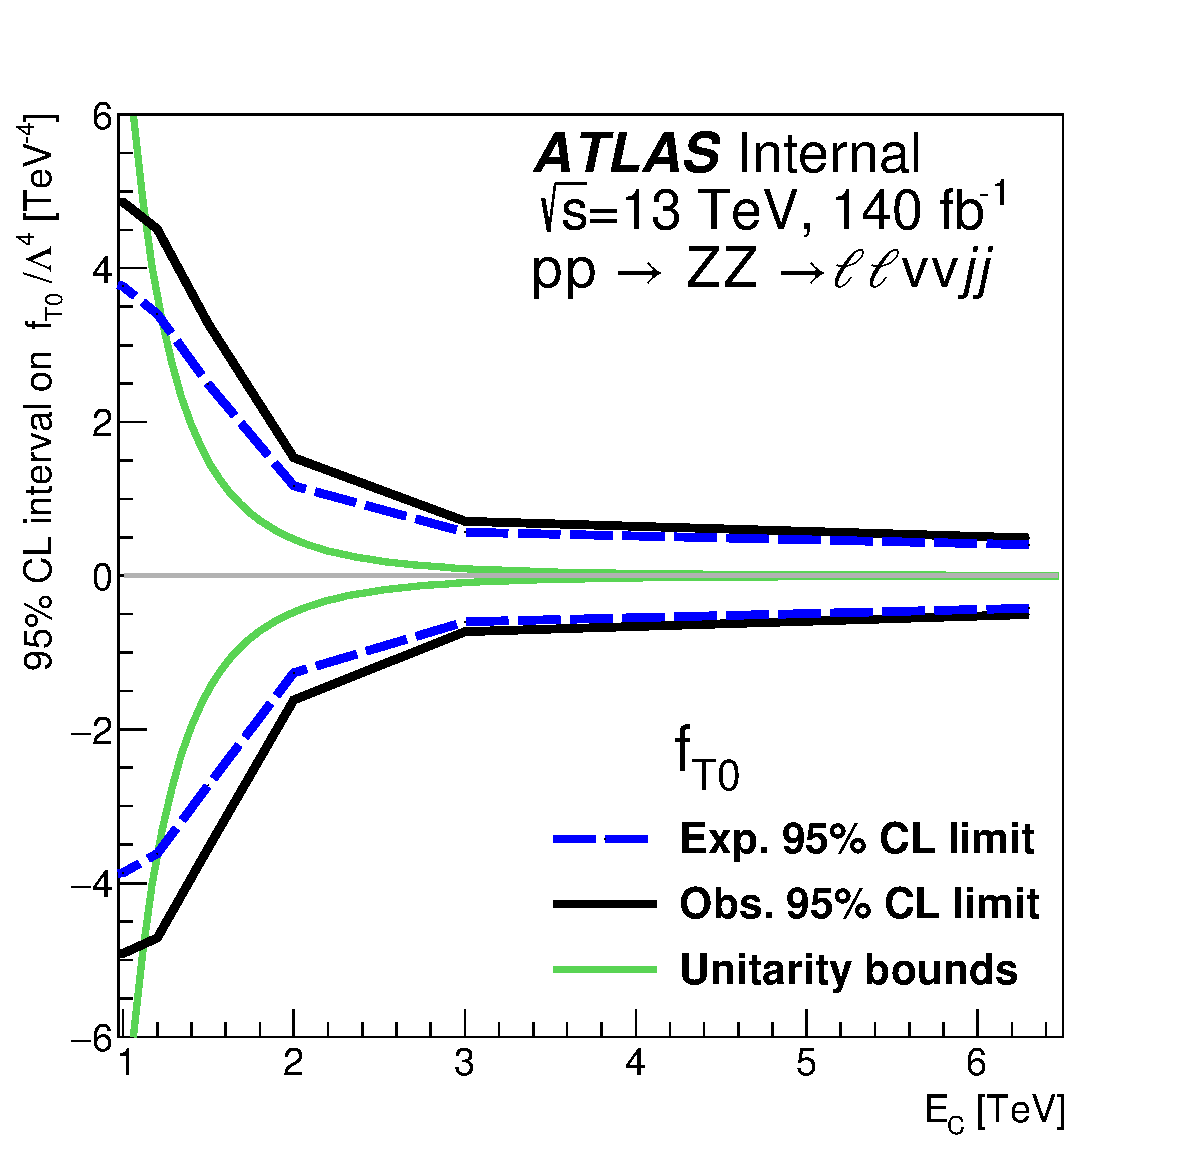
\includegraphics[width=0.45\linewidth]{figures/ch5-llvv/aTGC-aQGC/FT0.pdf}
        \label{fig:aqgc_fT0}
    }
    \hfill
    \subfloat[]{
        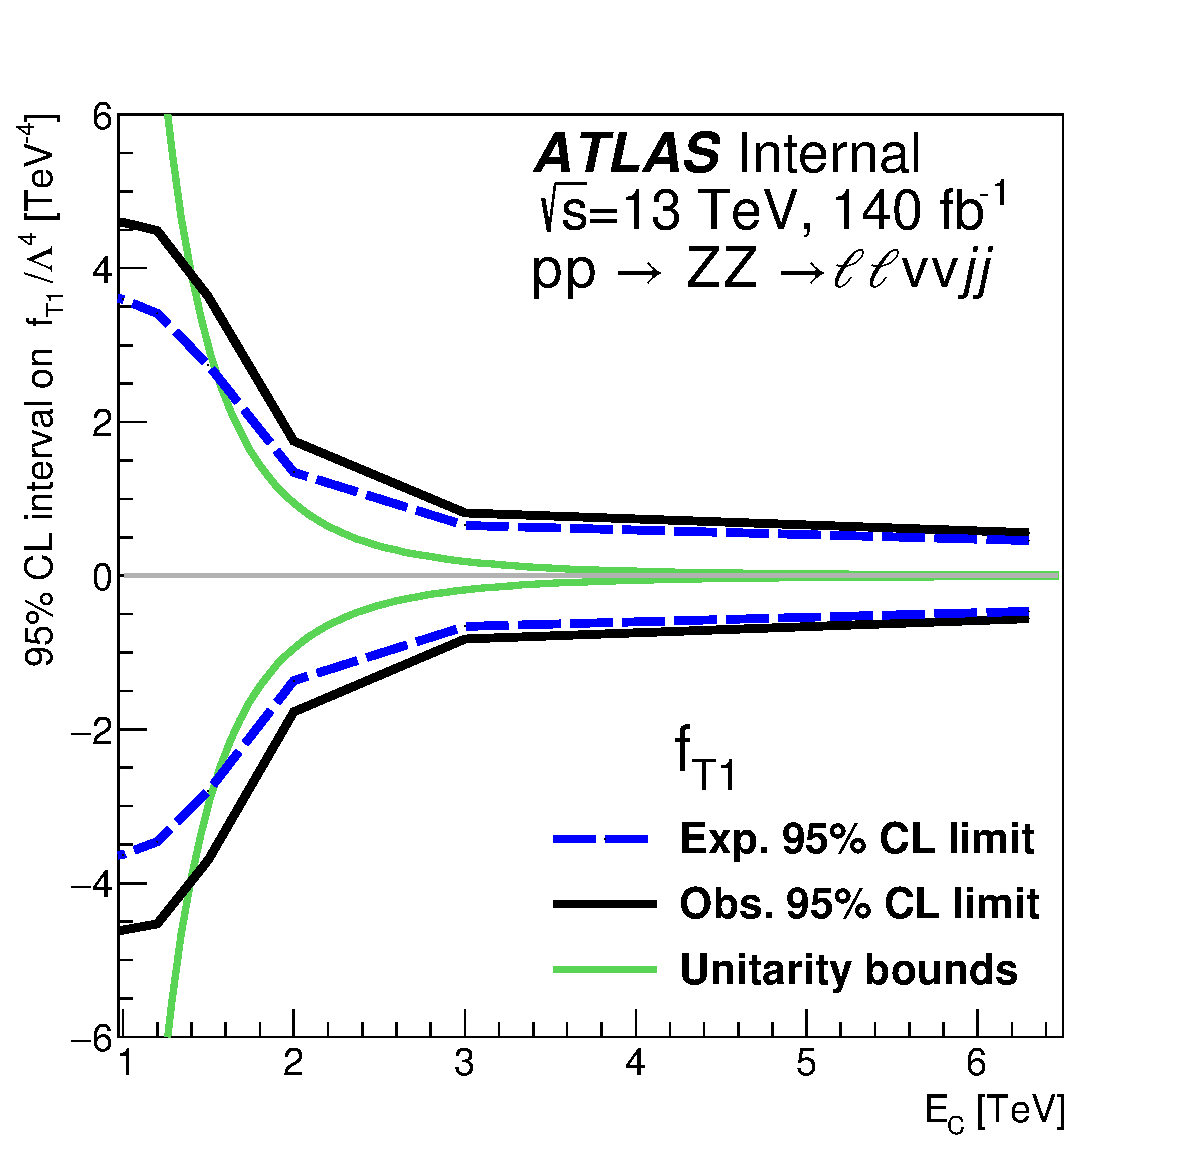
\includegraphics[width=0.45\linewidth]{figures/ch5-llvv/aTGC-aQGC/FT1.pdf}
        \label{fig:aqgc_fT1}
    }
    \\ % Line break for Bottom Row
    % Bottom Row: fT2 and fT3
    \subfloat[]{
        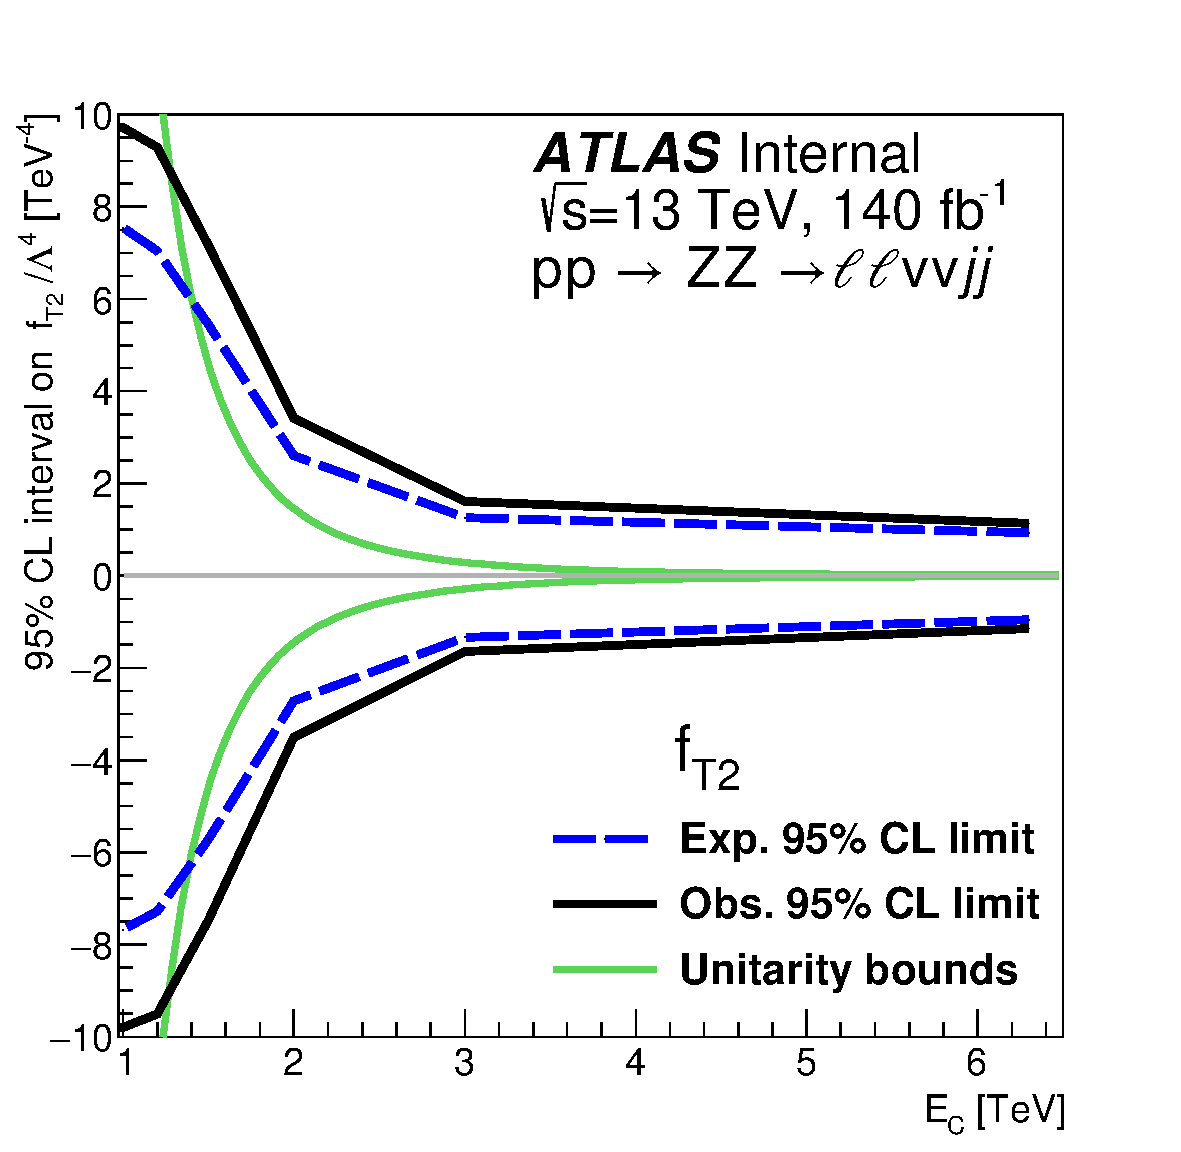
\includegraphics[width=0.45\linewidth]{figures/ch5-llvv/aTGC-aQGC/FT2.pdf}
        \label{fig:aqgc_fT2}
    }
    \hfill
    \subfloat[]{
        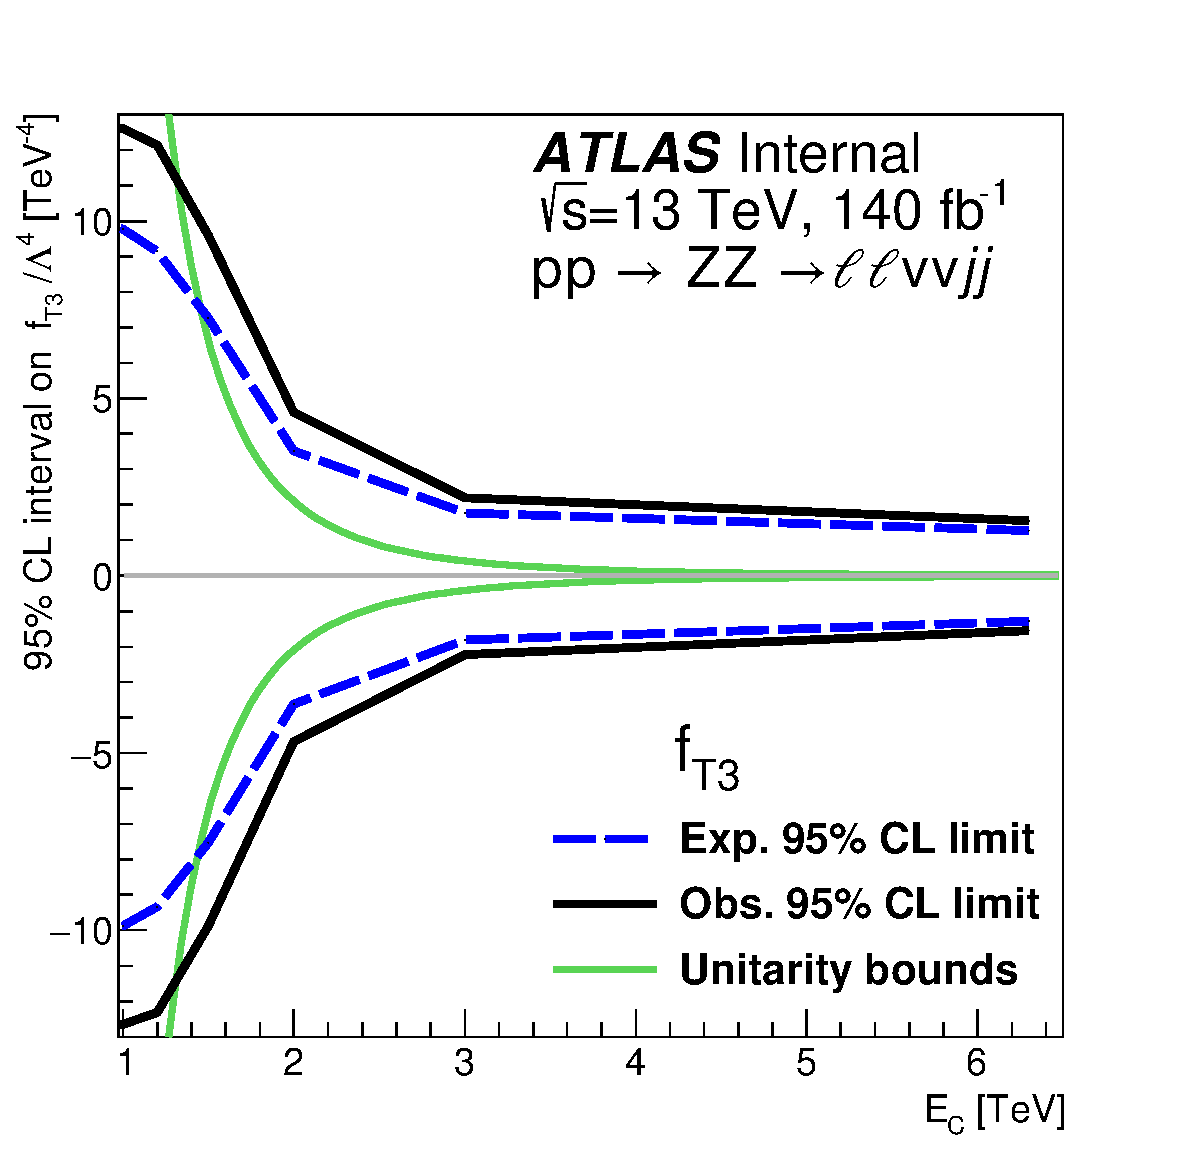
\includegraphics[width=0.45\linewidth]{figures/ch5-llvv/aTGC-aQGC/FT3.pdf}
        \label{fig:fT0-fT1_zzjj_EFT}
    }
    
    \caption{Expected and observed 95\% CL intervals for the Wilson coefficients (a) $f_{\text{T}0}$, (b) $f_{\text{T}1}$, (c) $f_{\text{T}2}$, and (d) $f_{\text{T}3}$ as a function of the EFT cut-off scale $E_{\text{c}}$. 
    The cut-off scale imposes a restriction such that the BSM amplitudes are set to zero when $m_{\text{ZZ}} > E_{\text{c}}$. 
    The dashed (solid) lines show the expected (observed) limits, and the solid green curve corresponds to the unitarity bounds.}
    \label{fig:aqgc_limits_fT0_fT3}
\end{figure}

\begin{figure}[!htbp]
    \centering
    \subfloat[]{
    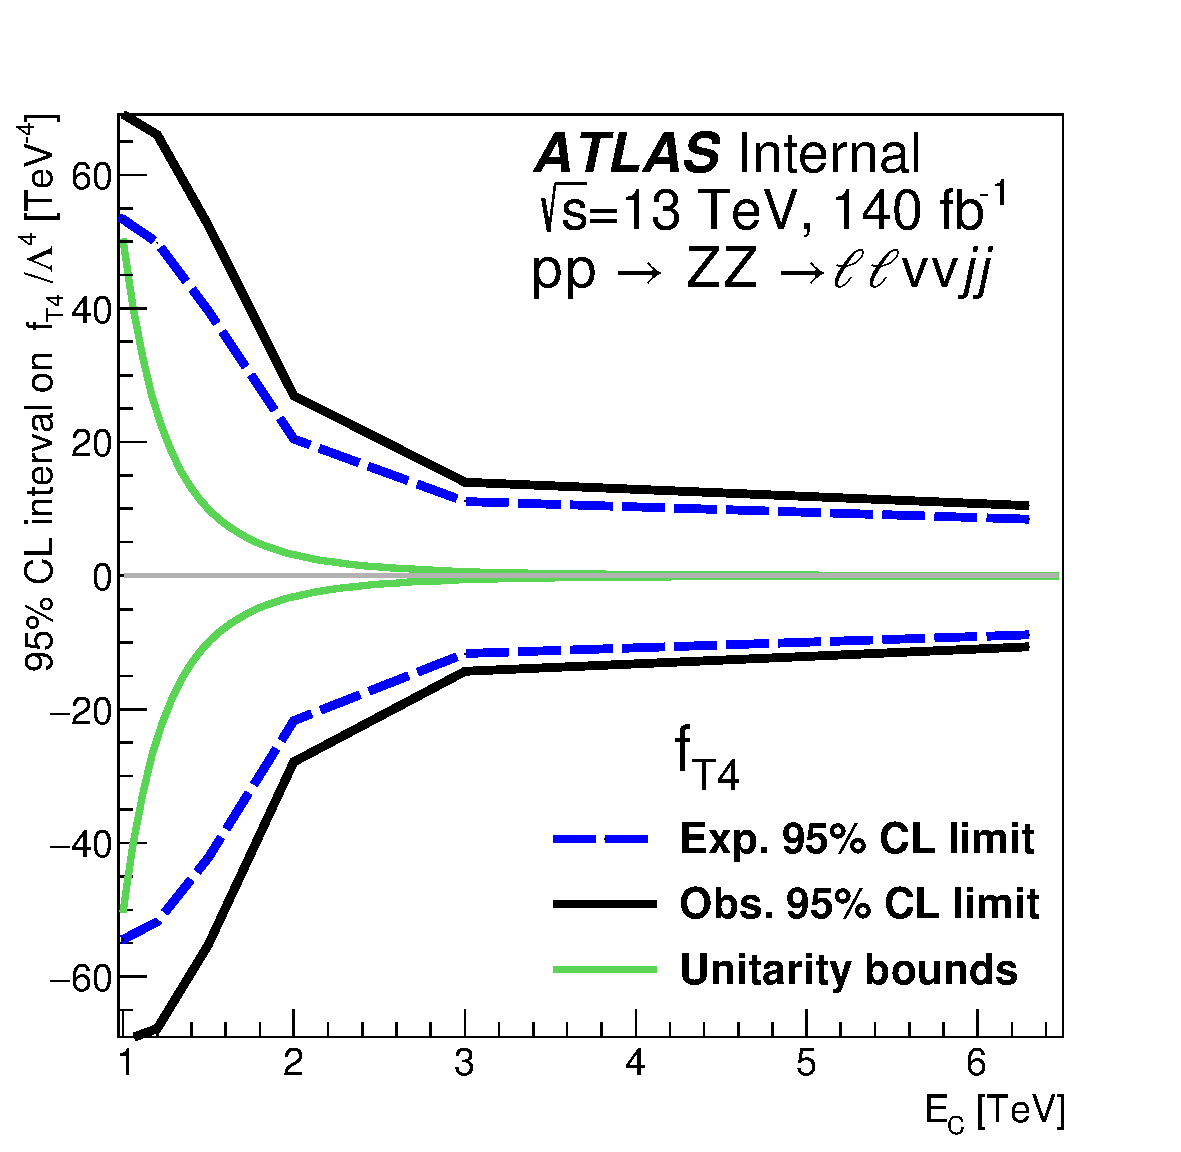
\includegraphics[width=0.45\linewidth]{figures/ch5-llvv/aTGC-aQGC/FT4.pdf}}
    \subfloat[]{
    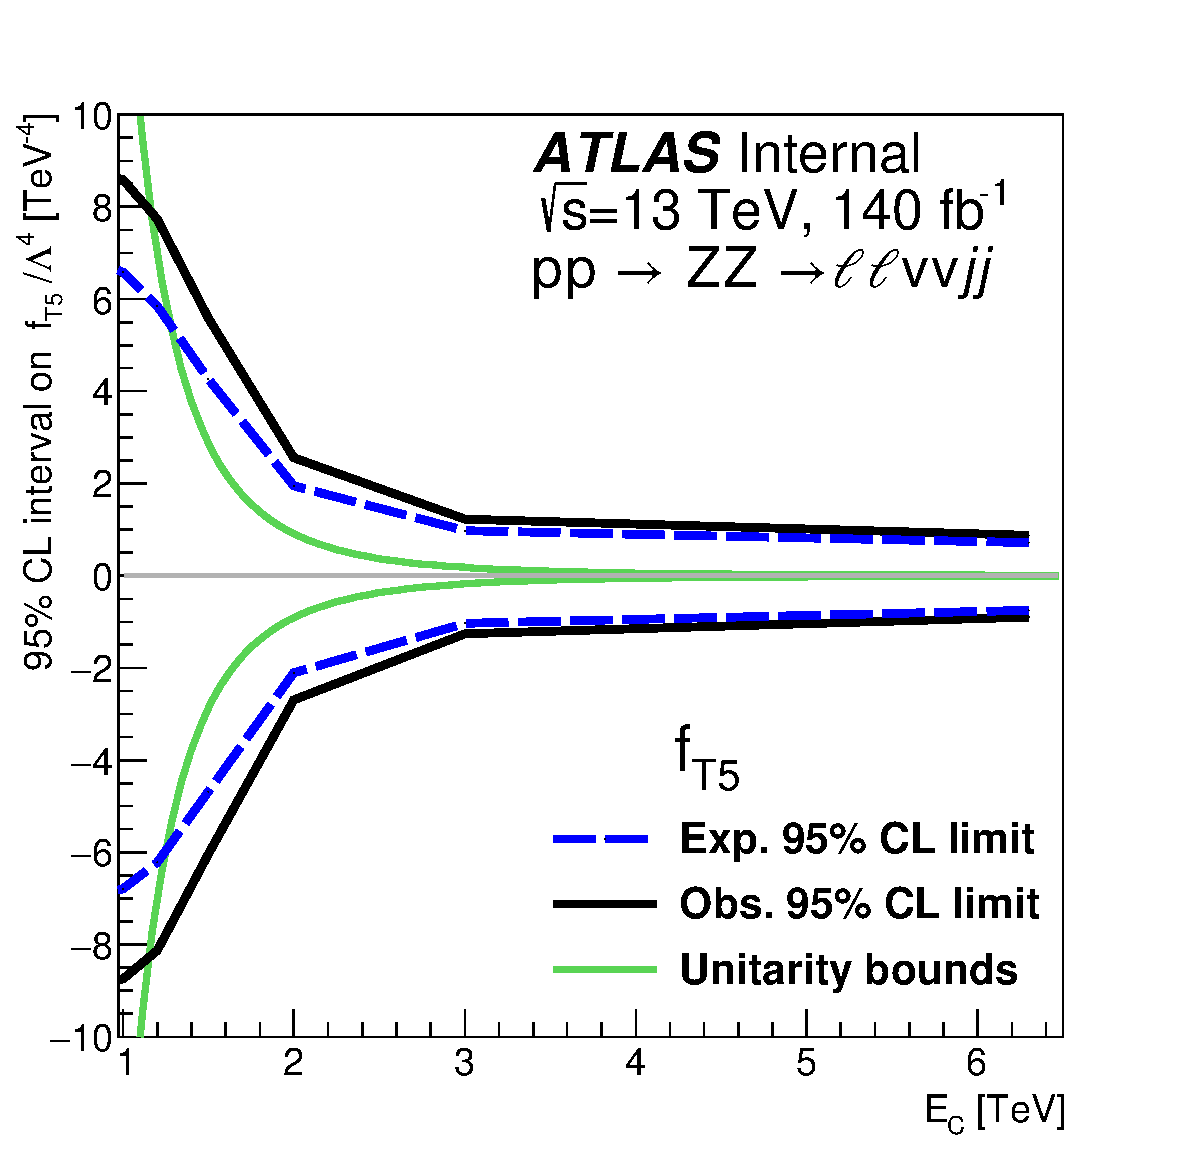
\includegraphics[width=0.45\linewidth]{figures/ch5-llvv/aTGC-aQGC/FT5.pdf}}
    \\
    \subfloat[]{
    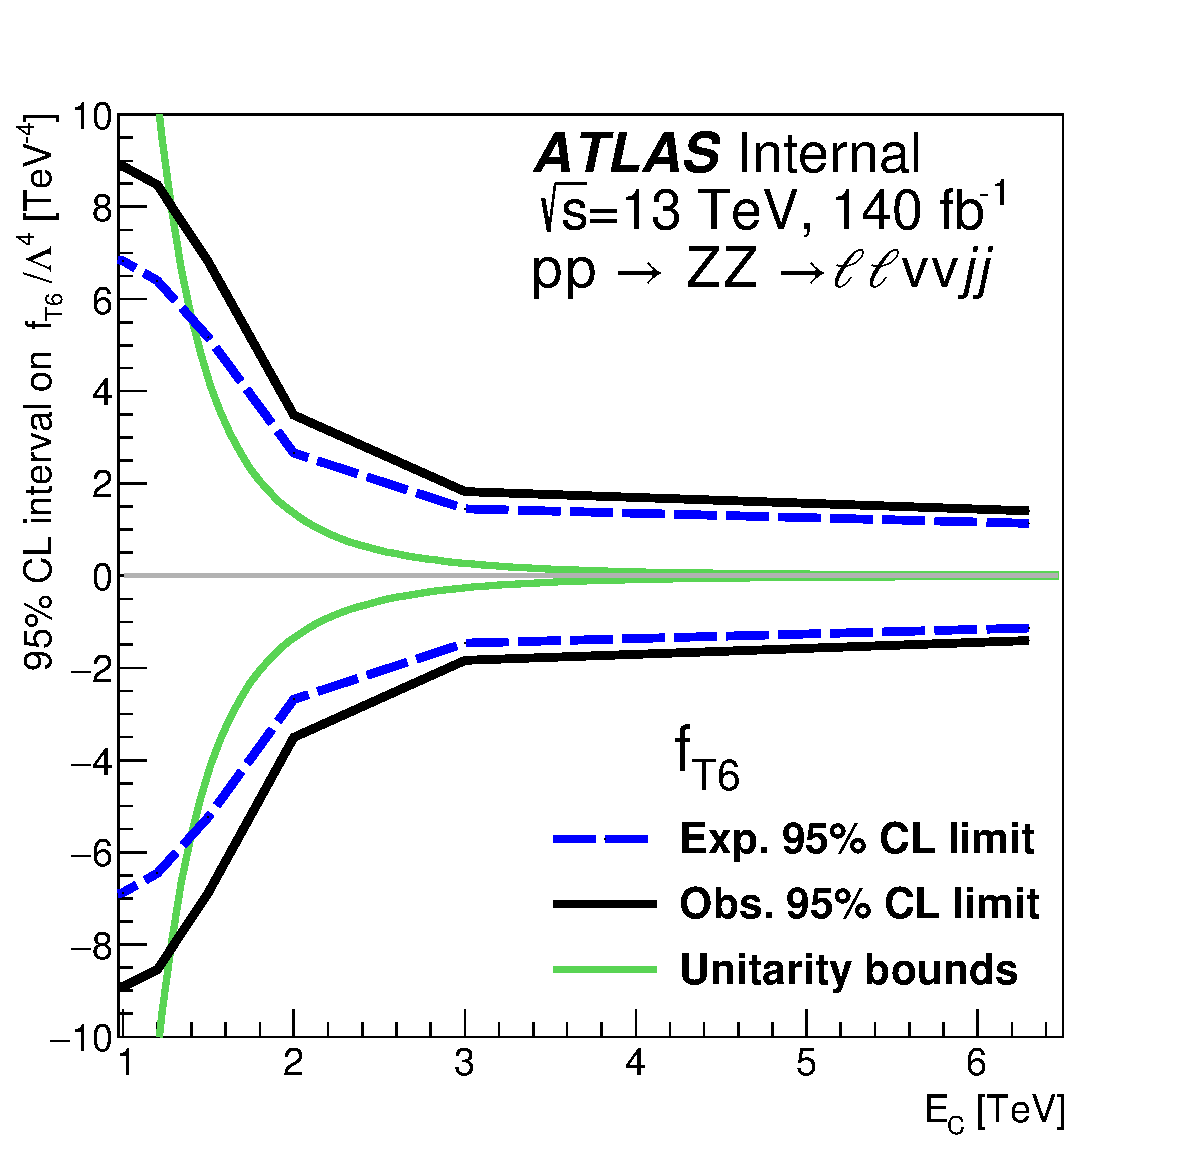
\includegraphics[width=0.45\linewidth]{figures/ch5-llvv/aTGC-aQGC/FT6.pdf}}
    \subfloat[]{
    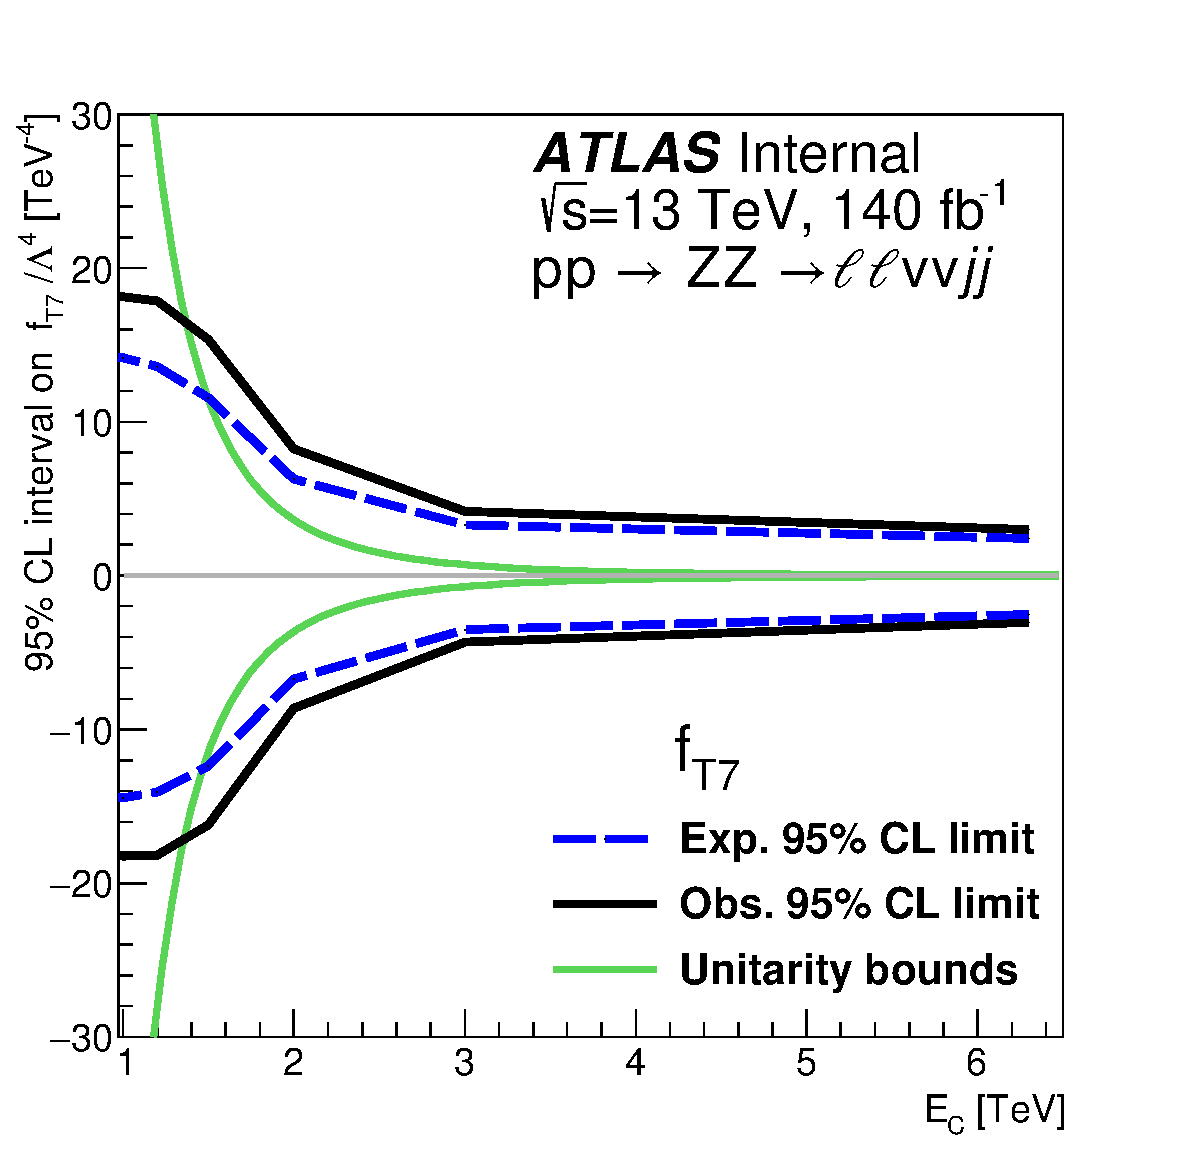
\includegraphics[width=0.45\linewidth]{figures/ch5-llvv/aTGC-aQGC/FT7.pdf}} 
    \\
    \subfloat[]{
    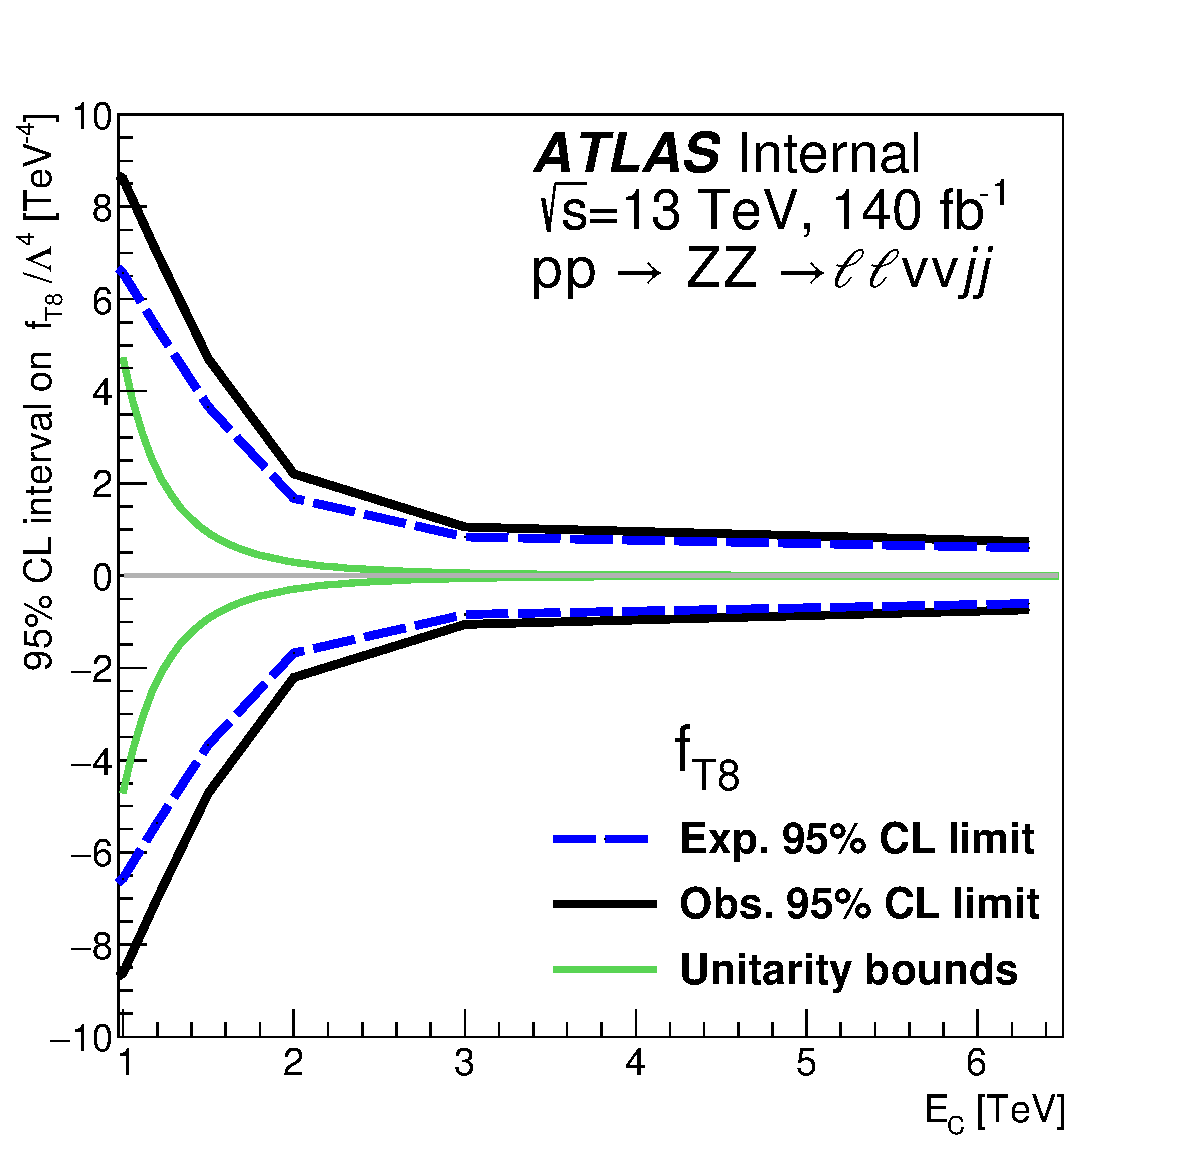
\includegraphics[width=0.45\linewidth]{figures/ch5-llvv/aTGC-aQGC/FT8.pdf}} 
    \subfloat[]{
    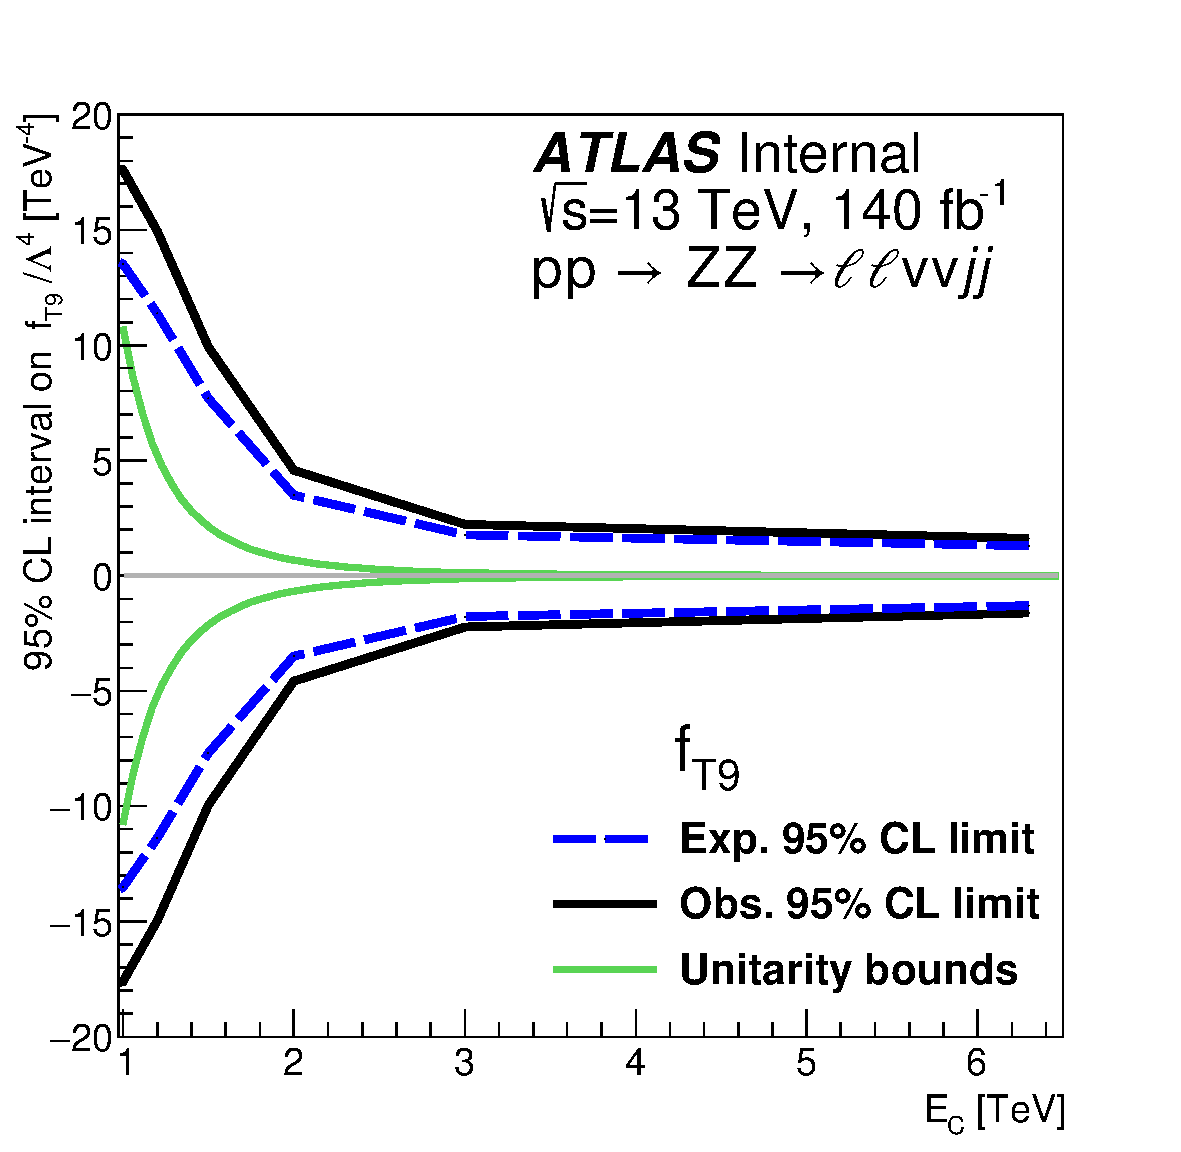
\includegraphics[width=0.45\linewidth]{figures/ch5-llvv/aTGC-aQGC/FT9.pdf}}
    \\
    \caption{The expected and observed 95\% CL for the $f_{\text{T}4}$ (a), $f_{\text{T}5}$ (b), $f_{\text{T}6}$ (c), $f_{\text{T}7}$ (d), $f_{\text{T}8}$ (e) and $f_{\text{T}9}$ (f) Wilson coefficients are derived as a function of the cut-off scale, $E_{\text{c}}$, which imposes a restriction such that the BSM amplitudes of interference and pure dimension-eight are set to zero when $m_{\text{ZZ}} > E_{\text{c}}$. 
These constraints are determined by performing a one-dimensional fit to the $m_{\text{T}}^{\text{ZZ}}$ distribution in the $\ell\ell\nu\nu jj$ signal region. 
The dashed (solid) lines show the expected (observed) 95\% CL limits, and the solid curve corresponds to the unitarity bounds~\cite{Almeida:2020ylr}.
 }
    \label{fig:fT2-fT9_zzjj_EFT}
\end{figure}


% \begin{figure}[htbp]
%     \centering
%     % Row 1
%     \subfloat[]{
%         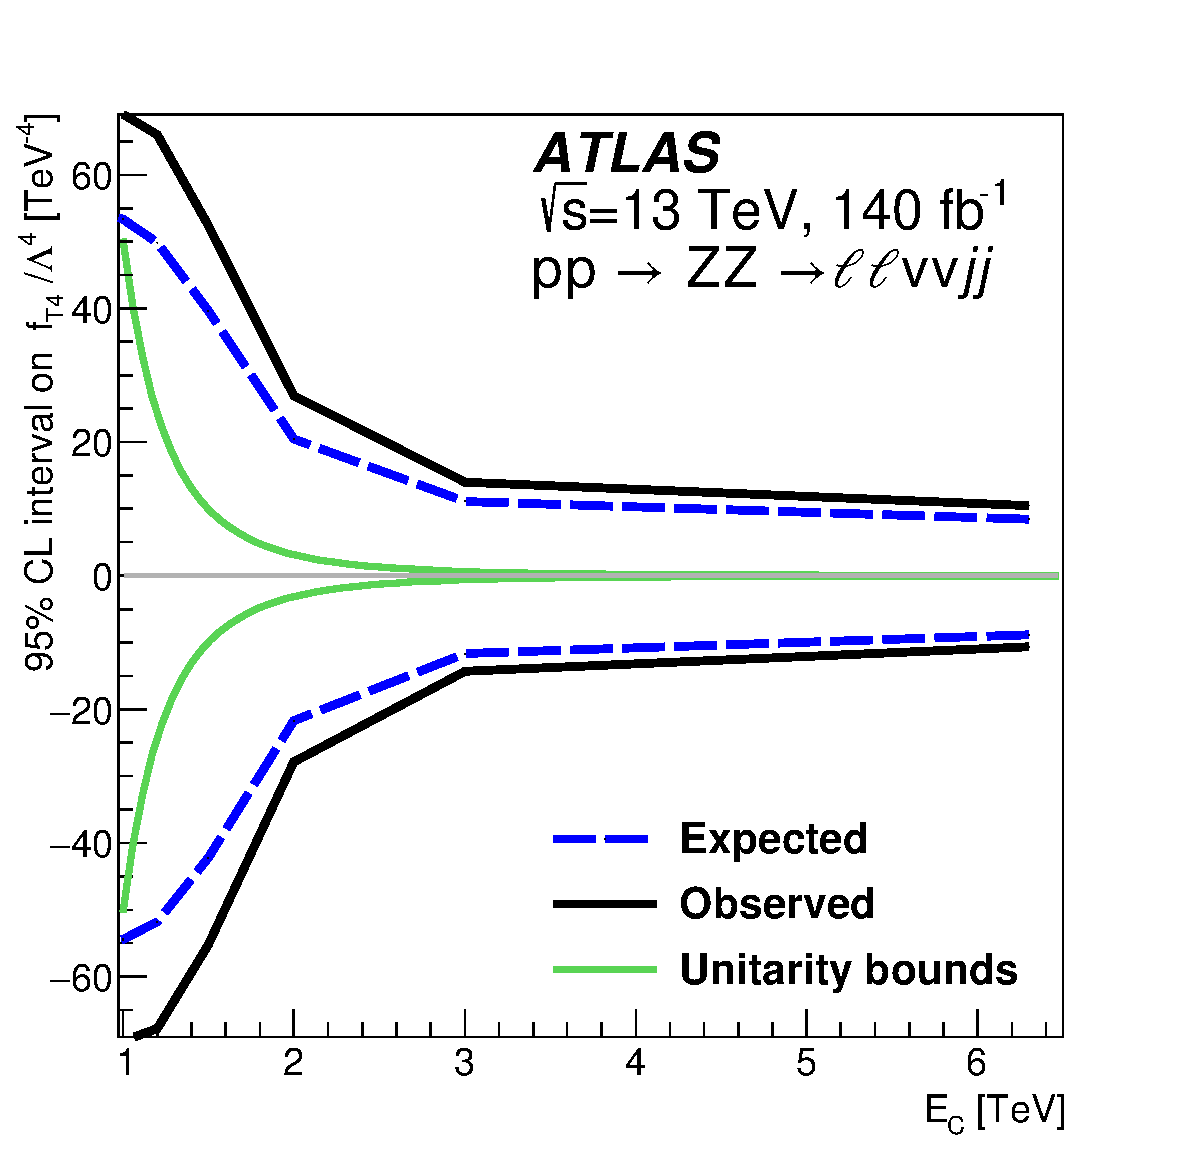
\includegraphics[width=0.32\textwidth]{figures/ch5-llvv/fig_aqgc_limit_fT4.pdf}
%         \label{fig:aqgc_fT4}
%     }
%     \hfill
%     \subfloat[]{
%         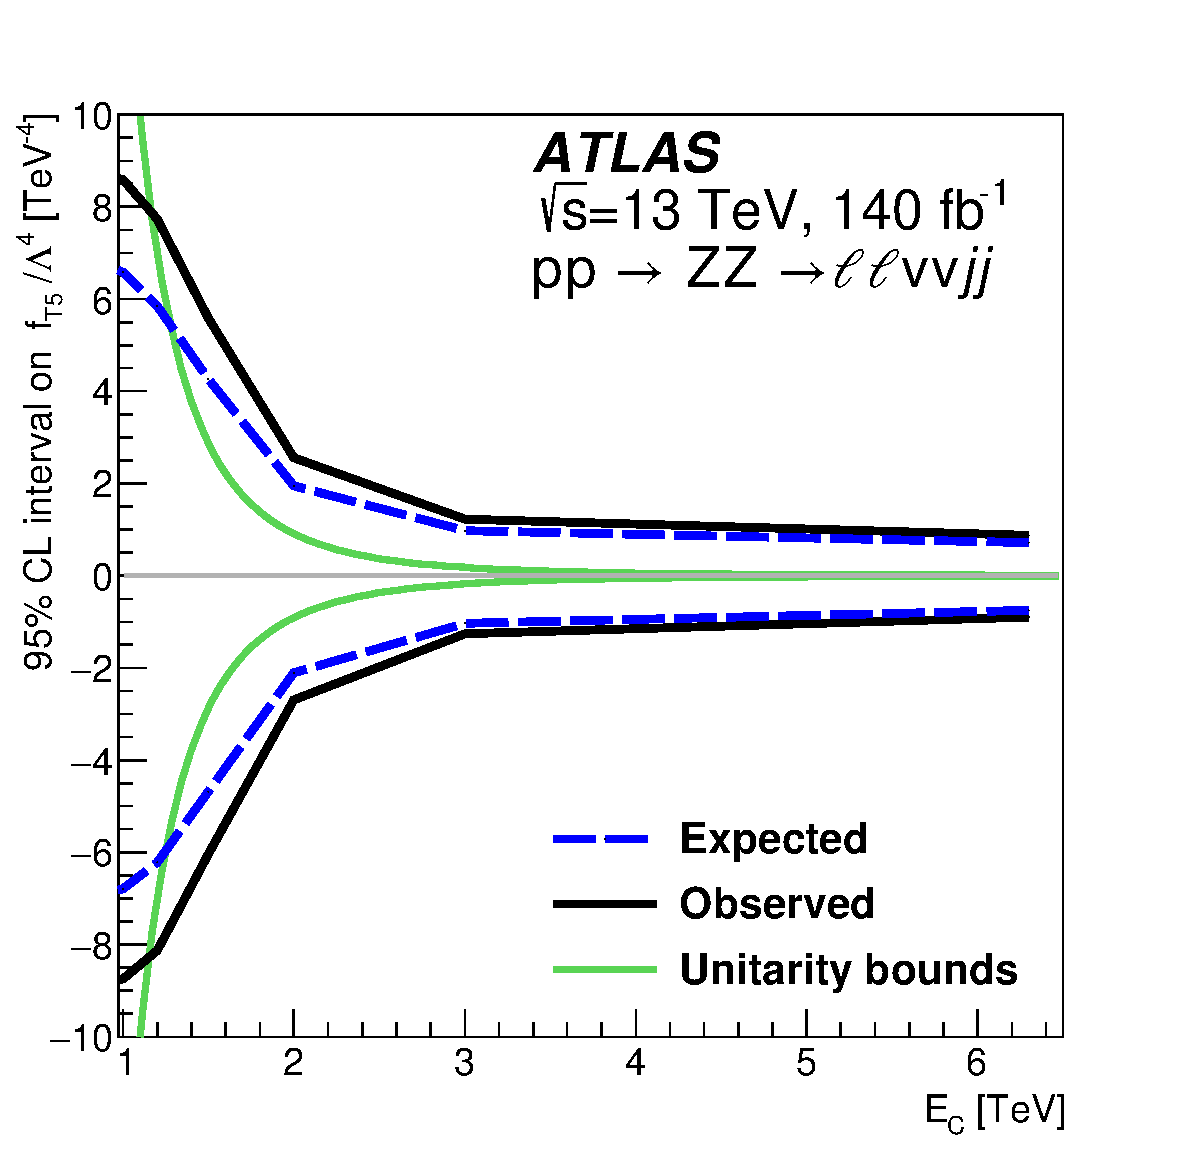
\includegraphics[width=0.32\textwidth]{figures/ch5-llvv/fig_aqgc_limit_fT5.pdf}
%         \label{fig:aqgc_fT5}
%     }
%     \hfill
%     \subfloat[]{
%         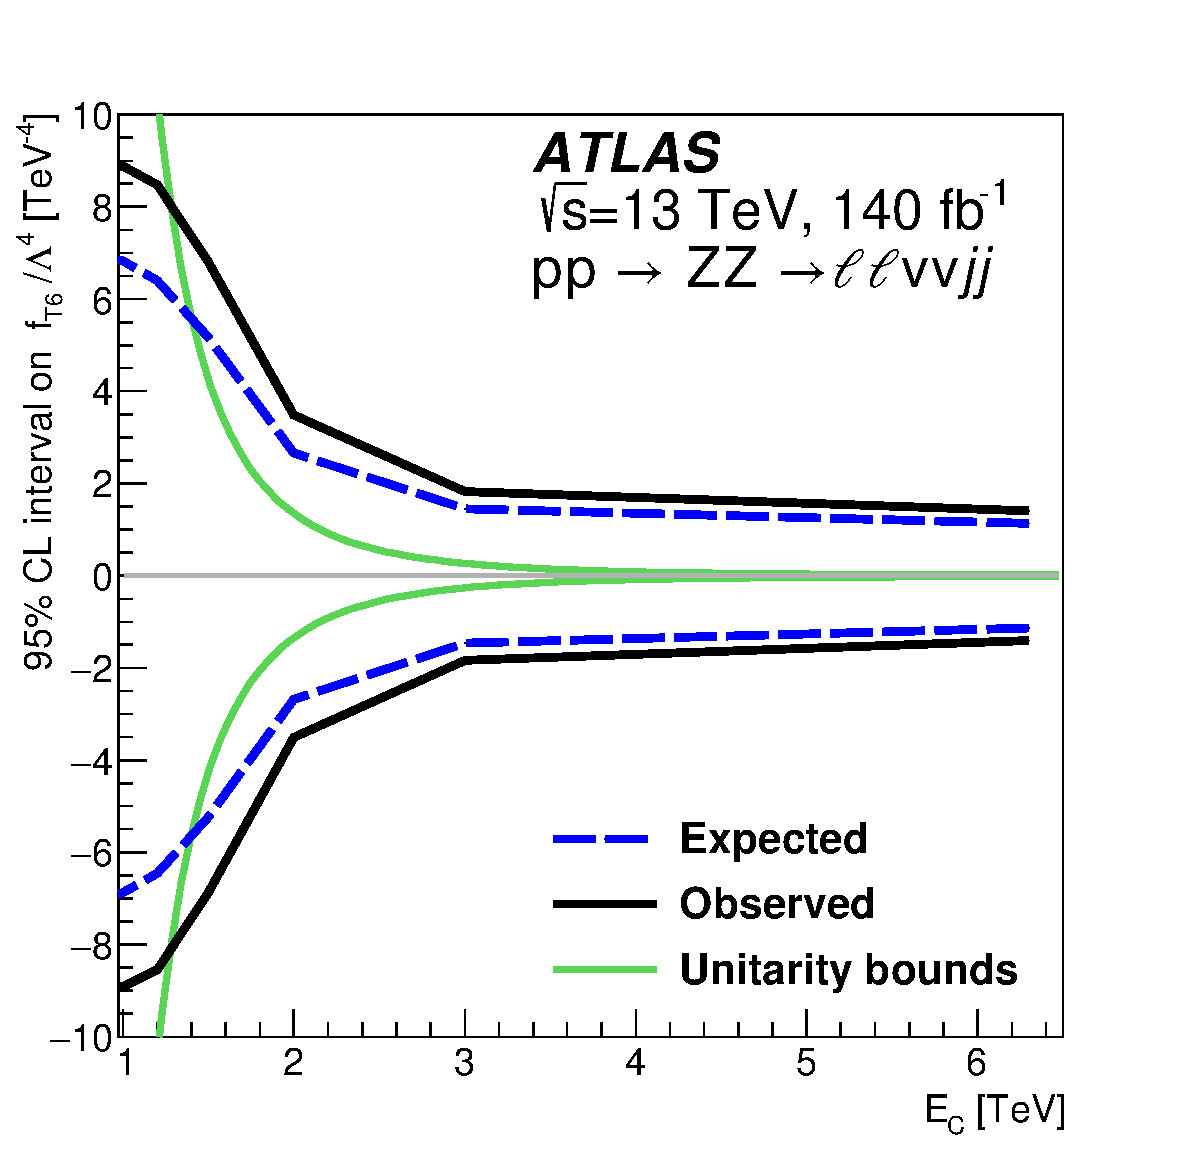
\includegraphics[width=0.32\textwidth]{figures/ch5-llvv/fig_aqgc_limit_fT6.pdf}
%         \label{fig:aqgc_fT6}
%     }
%     \\ % Line break
%     % Row 2
%     \subfloat[]{
%         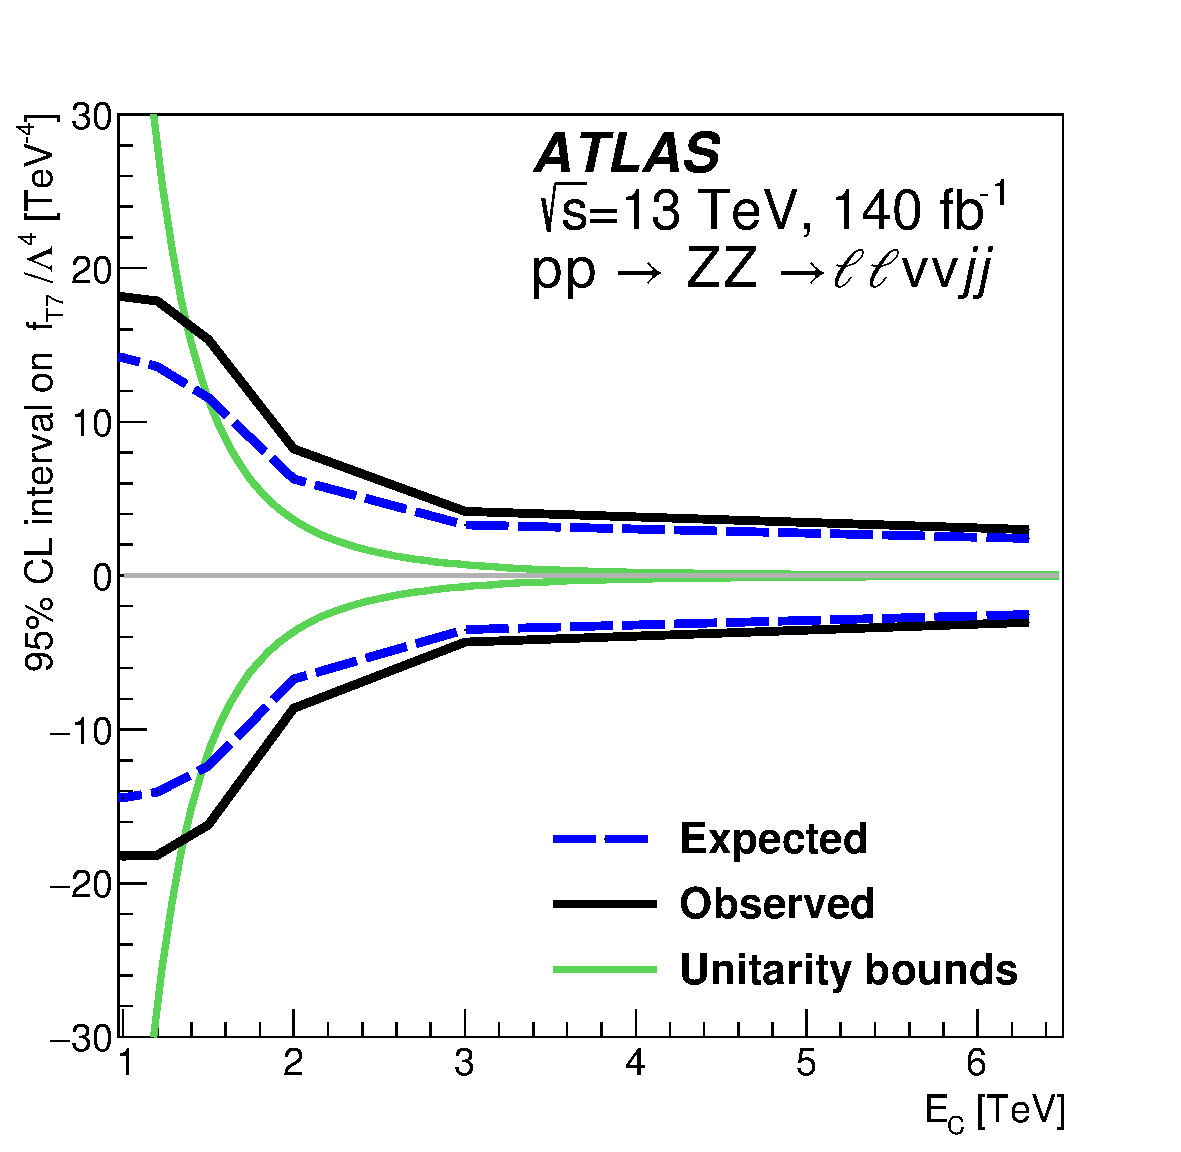
\includegraphics[width=0.32\textwidth]{figures/ch5-llvv/fig_aqgc_limit_fT7.pdf}
%         \label{fig:aqgc_fT7}
%     }
%     \hfill
%     \subfloat[]{
%         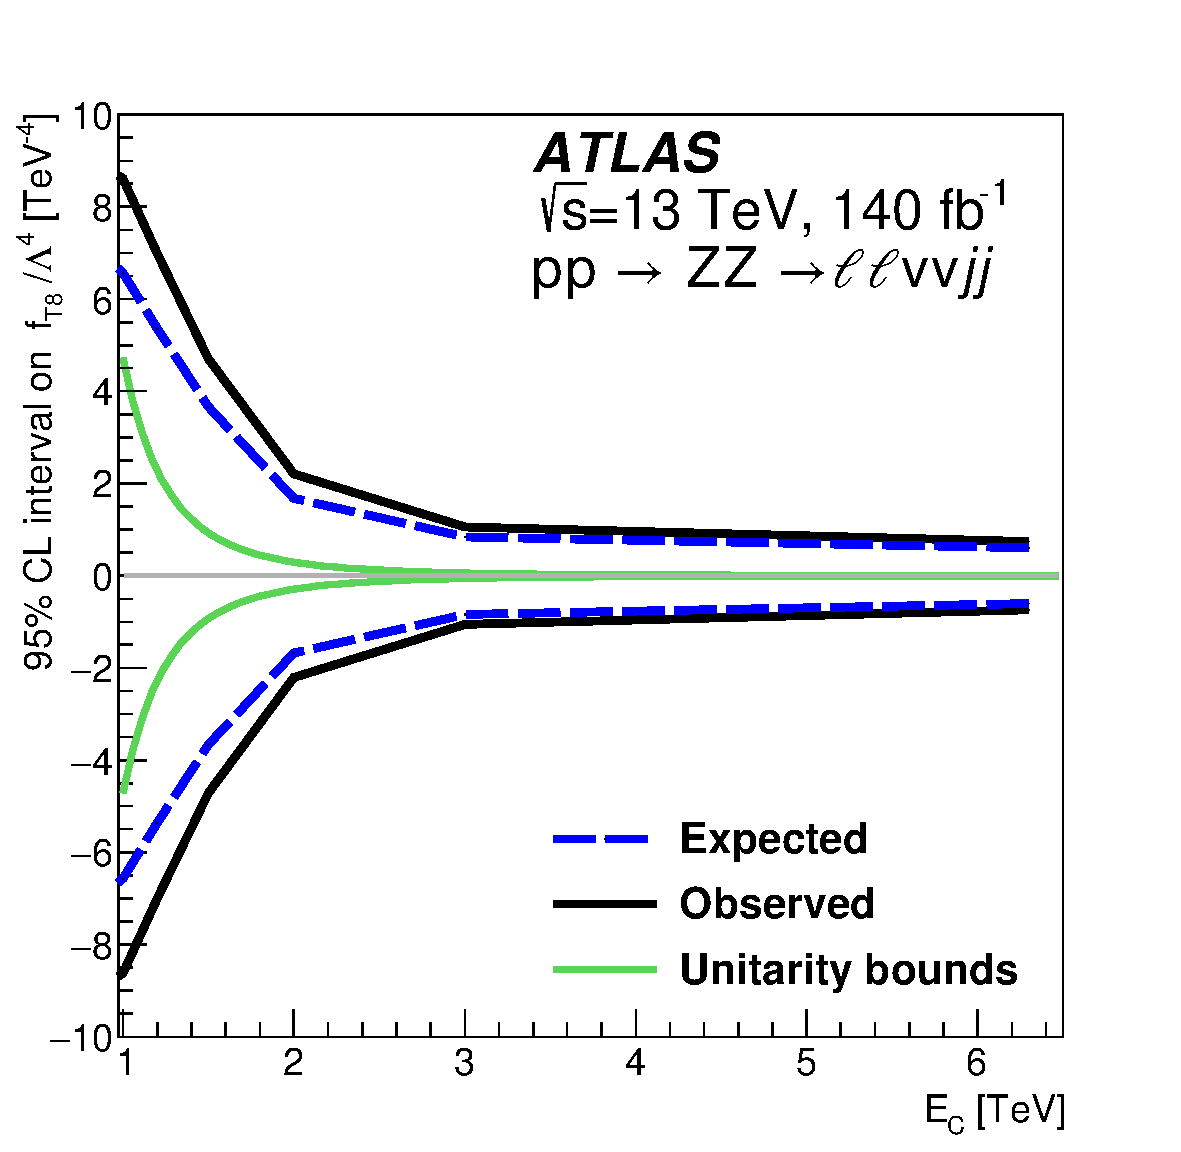
\includegraphics[width=0.32\textwidth]{figures/ch5-llvv/fig_aqgc_limit_fT8.pdf}
%         \label{fig:aqgc_fT8}
%     }
%     \hfill
%     \subfloat[]{
%         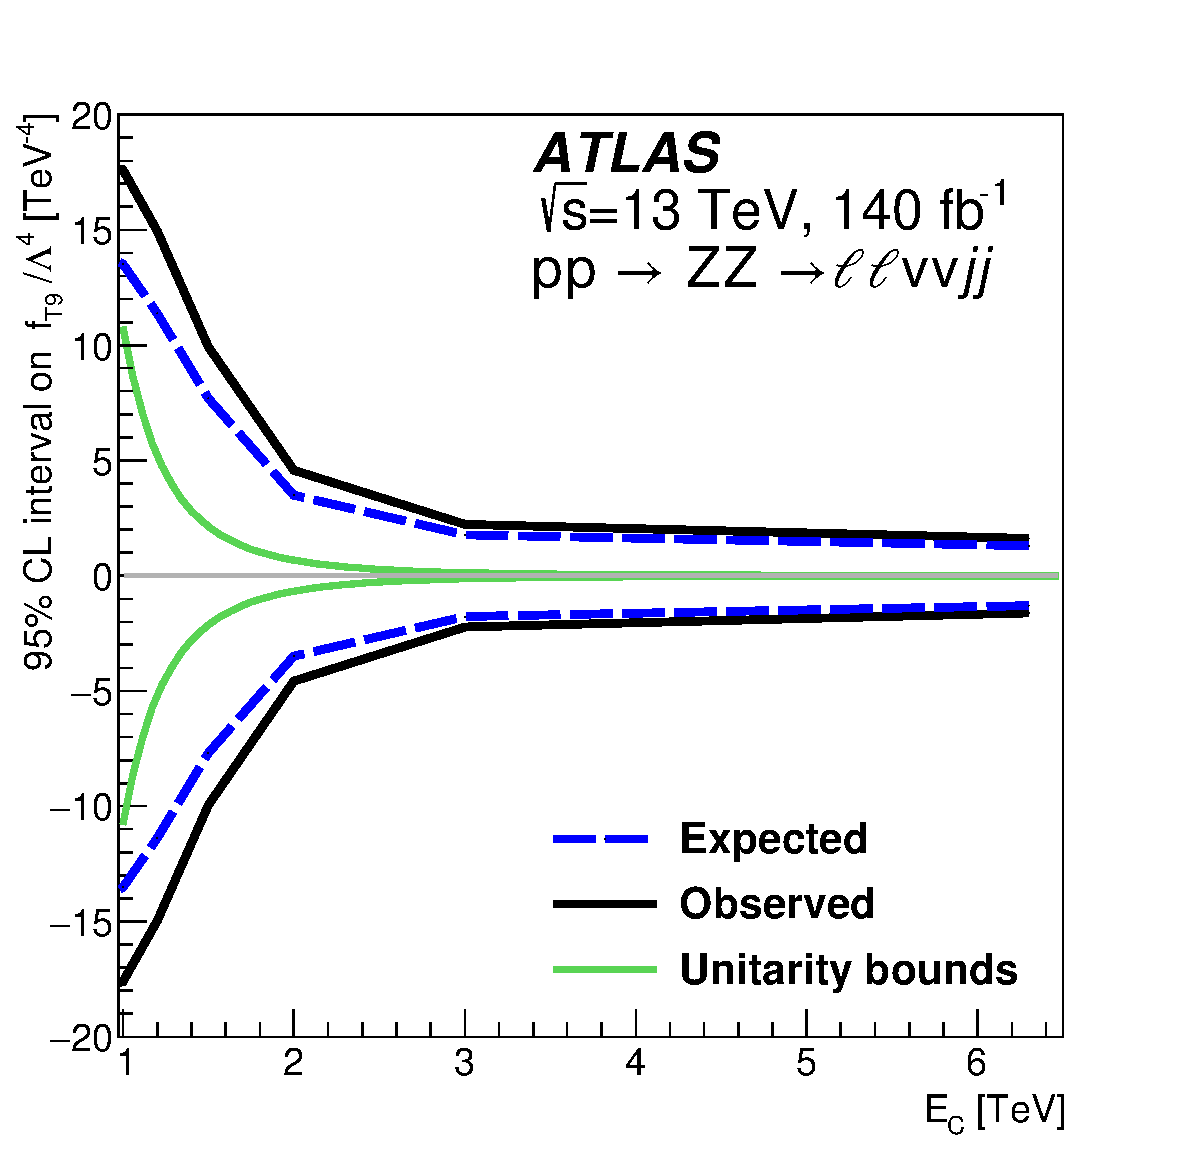
\includegraphics[width=0.32\textwidth]{figures/ch5-llvv/fig_aqgc_limit_fT9.pdf}
%         \label{fig:aqgc_fT9}
%     }
%     \caption{Expected and observed 95\% CL intervals for the Wilson coefficients $f_{\text{T}4}$ through $f_{\text{T}9}$ as a function of the EFT cut-off scale $E_{\text{c}}$. The dashed (solid) lines show the expected (observed) limits, and the solid green curve corresponds to the unitarity bounds.}
%     \label{fig:aqgc_limits_fT4_fT9}
% \end{figure}

\section{Summary of Results}

Integrated and differential cross-sections for $\text{Z}$ boson pair production in the 
$\text{ZZ} \to \ell^+\ell^- \nu\bar{\nu}$ final state are measured in both inclusive $\text{ZZ}$ and VBS-like $\text{ZZ}jj$ production modes at $\sqrt{s}=13~\text{TeV}$ using $140~\text{fb}^{-1}$ of ATLAS data. Stringent constraints are placed on neutral anomalous triple gauge couplings (aTGCs) and anomalous quartic gauge couplings (aQGCs) based on this analysis. 

The fiducial cross-sections for inclusive $\text{ZZ} \to \ell\ell\nu\nu$ and $\text{ZZ}jj \to \ell\ell\nu\nu jj$ production are measured to be $21 \pm 1~\text{fb}$ and $0.96^{+0.18}_{-0.16}~\text{fb}$, respectively, in agreement with the SM predictions of $20.1 \pm 1.1~\text{fb}$ and $0.94 \pm 0.20~\text{fb}$ from \textsc{Sherpa}+\textsc{MadGraph5} calculations. Compared with earlier measurements using a partial Run~2 dataset, the total uncertainty in the inclusive $\text{ZZ}$ fiducial cross-section is reduced from 7.0\% to 4.6\% and is now dominated by statistical uncertainty. The \textsc{Matrix} prediction for the inclusive fiducial cross-section is $21.03 \pm 0.30~\text{fb}$, reflecting improved theoretical precision from calculations including NNLO QCD and NLO electroweak corrections. The inclusive $\text{ZZ} \to \ell\ell\nu\nu$ cross-section extrapolated to the total phase space is measured to be $15.38 \pm 0.81~\text{pb}$, consistent with the SM prediction of $15.40 \pm 0.38~\text{pb}$ from \textsc{Matrix}.

Differential cross-sections for both $\text{ZZ}$ and $\text{ZZ}jj$ production are measured as functions of key kinematic observables, providing stringent tests of the SM and valuable inputs for modelling studies. The transverse momentum of the dilepton system is used to constrain anomalous neutral triple gauge couplings using both the vertex-function and SMEFT frameworks. In the vertex-function formalism, limits are set on $f_{4}^{\text{Z}}$, $f_{4}^{\gamma}$, $f_{5}^{\gamma}$, and $f_{5}^{\text{Z}}$, improving previous results in this final state by approximately a factor of 1.7. In the SMEFT interpretation, performed for the first time for this channel, limits are derived on Wilson coefficients associated with neutral aTGCs.

In the $\text{ZZ}jj$ channel, the transverse mass of the $\text{ZZ}$ system is used to constrain dimension-eight operators contributing to anomalous quartic gauge couplings. These results improve sensitivity by a factor of approximately 2--3 relative to the $4\ell jj$ channel, owing to the larger branching ratio of the $\ell\ell\nu\nu$ final state. Overall, the measurements show excellent agreement with SM predictions and significantly enhance sensitivity to physics beyond the SM in the electroweak sector.

%The fiducial and differential cross-sections for the inclusive $\text{ZZ} \to \ell\ell\nu\nu$ process have been measured with high precision using the full ATLAS Run 2 dataset. The inclusive fiducial cross-section is measured with a precision of 4.8\%, limited by statistics. All measurements show excellent agreement with SM predictions. 

%Stringent limits have been placed on anomalous triple gauge couplings, significantly constraining the phase space for new physics in the electroweak sector.